\newcommand{\utilizzo}{\item \textbf{Utilizzo nel progetto}}

\section{Design pattern utilizzati}
\label{pattern}
\subsection{Pattern architetturali}
	\subsubsection{Model View Controller}
	
		\begin{figure}[!h]
			\centering
			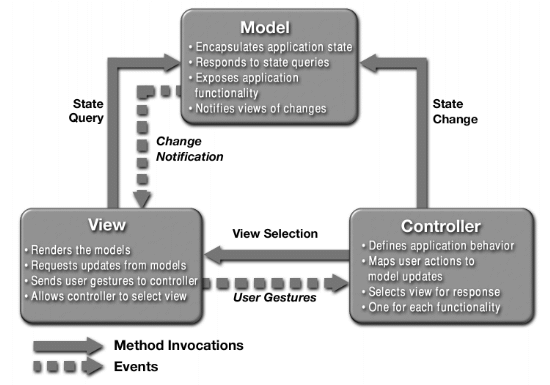
\includegraphics[scale=0.5]{img/mvc}  
			\caption{Struttura del pattern MVC}
		\end{figure}
		
		\begin{itemize}	
			\item \textbf{Descrizione} \\ Model View Controller è un design pattern architetturale che permette di dividere l'architettura del sistema che si intende sviluppare in tre blocchi:
			\begin{itemize}
				\item \textbf{il modello} che contiene le classi con i metodi di accesso ai dati;
				\item \textbf{la vista} che contiene le classi che permettono all'utente di visualizzare i dati e di interagire con il modello;
				\item \textbf{il controllore} che si occupa di fare da tramite tra vista e modello, ovvero riceve i comandi dell'utente attraverso la vista e va a cambiare lo stato del modello di conseguenza, successivamente aggiorna la vista.				
			\end{itemize}
			% immagine generale
			
			\item \textbf{Vantaggi} \\
			Questo pattern architetturale permette il riuso del codice in quanto molte parti di lavoro sono indipendenti. Ad esempio il modello creato potrà essere utilizzato con diverse viste. \\ Grazie all'indipendenza di alcune parti è semplice dividere il lavoro tra più componenti di un team e sarà quindi più facile anche la manutenzione.
			\utilizzo \\
			Nel nostro progetto il pattern MVC è usato nella parte client dell'architettura. 
		\end{itemize}
		
\subsection{Pattern creazionali}
	\subsubsection{Abstract Factory}
	
	\begin{figure}[!h]
		\centering
		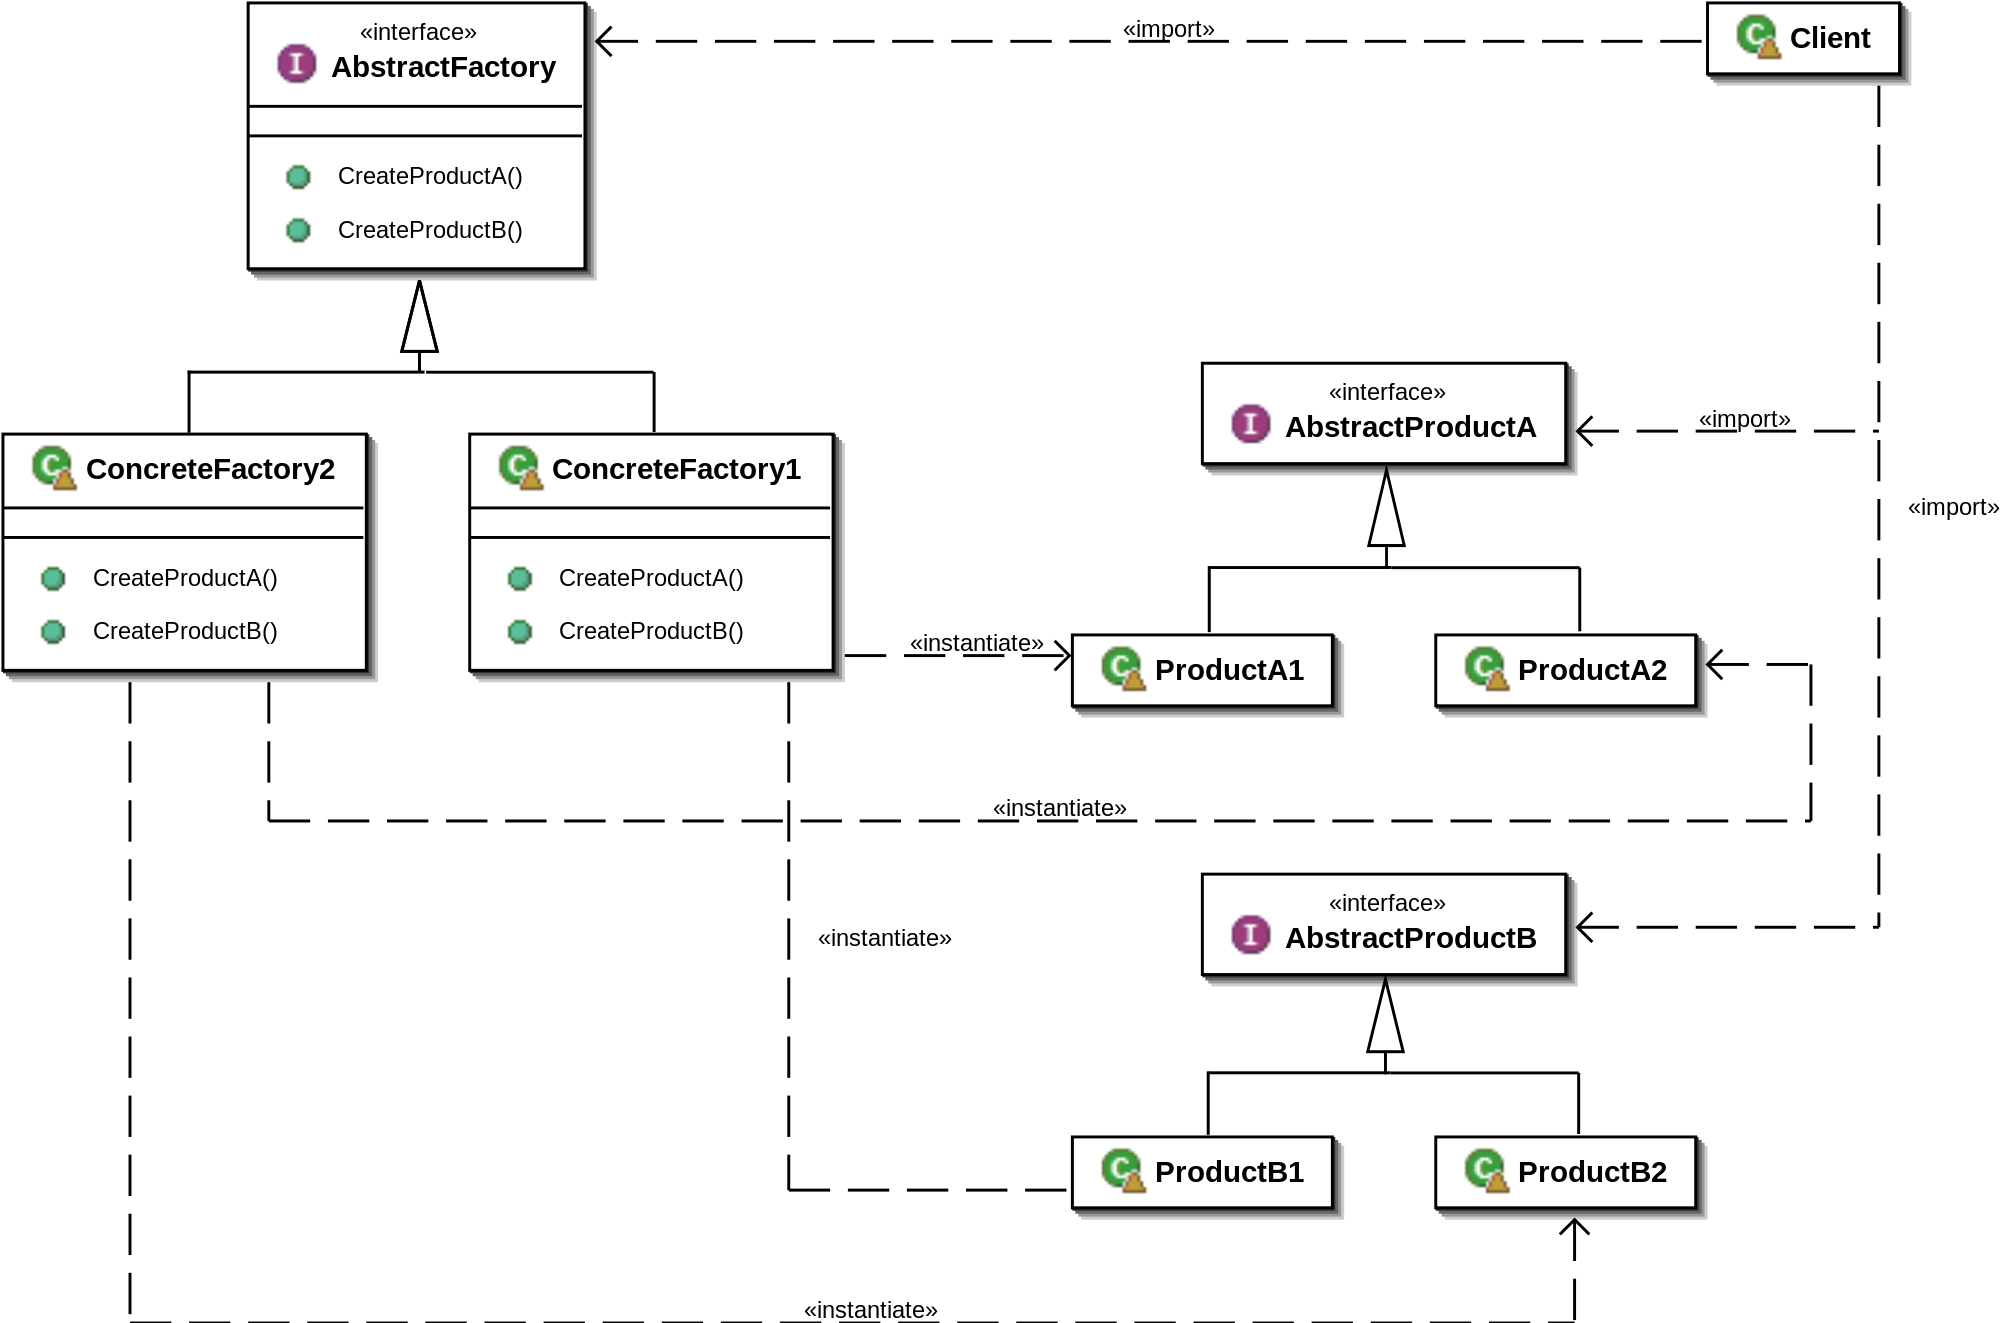
\includegraphics[scale=0.2]{img/abstract_factory}  
		\caption{Struttura del pattern Abstract Factory}
	\end{figure}
	
		\begin{itemize}
			\item \textbf{Descrizione}\\ 
			Il design pattern Abstract Factory fornisce un'interfaccia per creare famiglie di prodotti senza specificare classi concrete. Ogni famiglia di prodotti ha una classe base astratta da cui derivano delle classi concrete. Queste classi concrete sono istanziate dalle classi concrete della factory corrispondenti.
			% immagine d esempio
			
			\item \textbf{Vantaggi}\\ 
			Questo design pattern offre vantaggi quando si vogliono modellare famiglie di prodotti che potranno essere ampliate nel futuro. Le modifiche necessarie ad aggiungere nuovi elementi alle famiglie saranno essenzialmente due, aggiungere una classe in ogni famiglia di prodotti ed un solo metodo nella factory.
			\utilizzo \\ 
			Nel nostro progetto abbiamo utilizzato questo design pattern per modellare i tipi di quiz che vengono proposti agli utenti. Abbiamo infatti deciso di utilizzare solo due famiglie di quiz, quindi vi è la necessità di avere modo in futuro di ampliare le tipologie di quiz disponibili in modo semplice ed efficace.
			
			% immagine diagramma nostro
		\end{itemize}
		
